\chapter{Diseño}

\section{Arquitectura conceptual propuesta}
\label{sec:arquitectura_propuesta}

La arquitectura de la Figura~\ref{fig:arquitectura_diseno} separará reglas, interpretación, representación, generación de sucesores y decisión mediante el modelo formal de la Sección~\ref{sec:modelo_formal_juego}. El contorno delimitará el núcleo reutilizable; las entradas y la coordinación de la partida quedarán fuera. Se trata de un diseño conceptual, sin fijar tecnología ni acreditar módulos implementados.

\begin{figure}[p]
\centering
\begin{tikzpicture}[
    bloque/.style={draw, rounded corners=3pt, align=center, text width=3.15cm, minimum height=1.15cm, inner sep=5pt, font=\small},
    externo/.style={bloque, fill=green!7, draw=green!45!black},
    interno/.style={bloque, fill=blue!5, draw=blue!55!black},
    flecha/.style={-{Stealth}, thick, draw=gray!80!black},
    consulta/.style={-{Stealth}, thick, draw=blue!65!black},
    etiqueta/.style={font=\footnotesize, align=center, fill=white, inner sep=2pt}
]
\node[externo] (reglas) at (0,0) {\textbf{Reglas externas}\\Gato o Ajedrez\\GDL o subconjunto\\o DSL por definir};
\node[interno] (interprete) at (5.2,0) {\textbf{Intérprete}\\Análisis léxico\\y sintáctico\\Validación\\de restricciones};
\node[interno] (modelo) at (10.4,0) {\textbf{Modelo interno $\Gamma$}\\Reglas y $s_0$\\Representación\\de estados};

\node[externo] (accion) at (0,-4.2) {\textbf{Acción elegida $a_i^*$}\\Acción legal para el rol\\activo, si $s\notin F$};
\node[interno, fill=orange!9] (motor) at (5.2,-4.2) {\textbf{Motor de decisión}\\Minimax / alfa-beta\\o MCTS / UCT\\(por seleccionar)\\Búsqueda si $s\notin F$};
\node[interno] (generador) at (10.4,-4.2) {\textbf{Consultas y generador}\\Acciones $L_i(s)$\\Sucesores $T(s,\mathbf a)$\\Terminalidad $s\in F$\\Utilidades $G_i(s)$};

\node[externo] (aplicar) at (0,-10.0) {\textbf{Aplicación en la partida}\\Consultar $T(s,\mathbf a^*)$\\Actualizar turno};
\node[externo] (estado) at (5.2,-10.0) {\textbf{Entrada por turno}\\Estado actual $s$\\Rol $r_i$ y presupuesto\\Inicialmente $s=s_0$};
\node[externo] (fin) at (10.4,-10.0) {\textbf{Fin de la partida}\\Si el estado actual $s\in F$\\Reportar $G_i(s)$\\Sin continuar la búsqueda};
\node[externo, fill=red!5, draw=red!45!black] (error) at (0,2.35) {\textbf{Diagnóstico}\\Descripción rechazada};

\begin{scope}[on background layer]
\node[draw=blue!55!black, dashed, rounded corners=5pt, fit=(interprete) (modelo) (motor) (generador), inner sep=9pt] (nucleo) {};
\end{scope}
\node[anchor=south east, font=\small\bfseries, text=blue!55!black] at ([yshift=3pt]nucleo.north east) {Núcleo reutilizable entre juegos};

\draw[flecha] (reglas) -- node[etiqueta, text width=1.25cm] {texto de reglas} (interprete);
\draw[flecha] (interprete) -- node[etiqueta, text width=1.25cm] {reglas\\válidas} (modelo);
\draw[flecha] (interprete.north) -- (5.2,2.35) -- node[etiqueta, above] {rechazo} (error.east);
\draw[flecha] (modelo) -- node[etiqueta, left, text width=2.0cm] {reglas\\consultables} (generador);
\draw[consulta] ([yshift=5pt]motor.east) -- node[etiqueta, above] {solicitudes} ([yshift=5pt]generador.west);
\draw[consulta] ([yshift=-5pt]generador.west) -- node[etiqueta, below] {resultados} ([yshift=-5pt]motor.east);
\draw[flecha] (motor) -- node[etiqueta] {elige} (accion);
\draw[flecha] (accion) -- node[etiqueta, right, text width=1.65cm] {solo la acción elegida} (aplicar);
\draw[flecha] (aplicar) -- node[etiqueta, text width=1.25cm] {estado sucesor} (estado);
% La coordinación usa el mismo servicio T que las consultas de búsqueda.
\draw[consulta] (aplicar.north east) -- (2.4,-6.5) --
    node[etiqueta, above, pos=0.15] {solicitar $T$ real}
    (10.0,-6.5) -- ([xshift=-4pt]generador.south);
\draw[consulta] ([xshift=4pt]generador.south) -- (10.6,-7.2) --
    node[etiqueta, below, pos=0.15] {partida: devolver $s'$}
    (2.0,-7.2) -- (aplicar.north);
% El trazo blanco distingue los cruces de líneas sin conexión.
\draw[flecha, preaction={draw=white,line width=4pt}] (estado) -- (motor);
\draw[flecha] (modelo.east) -- (12.7,0) -- (12.7,-11.7) --
    node[etiqueta, below, pos=0.5] {$s_0$: solo al cargar el juego}
    (5.2,-11.7) -- (estado.south);
\draw[flecha, preaction={draw=white,line width=4pt}] (motor.south east) -- (7.1,-5.9) -- (7.1,-8.3) -- node[etiqueta, above] {$s\in F$} (fin.north west);
\end{tikzpicture}
\caption{Arquitectura propuesta: carga de reglas, consultas de búsqueda y actualización de la partida. Las dos filas principales forman un único flujo; las entradas, salidas y condiciones de terminación se muestran alrededor del núcleo.}
\label{fig:arquitectura_diseno}
\end{figure}

\begin{enumerate}
    \item \textbf{Descripción externa.} Cada archivo expresará roles, estado inicial, acciones, legalidad, transiciones, terminalidad y utilidades. La elección del lenguaje requerirá justificar expresividad, restricciones y costo de interpretación.
    \item \textbf{Intérprete.} Analizará la estructura y las restricciones semánticas acordadas. La descripción aceptada originará el modelo; el rechazo producirá un diagnóstico y detendrá la carga.
    \item \textbf{Modelo y generador.} El modelo conservará las reglas y la representación de estados; el generador resolverá consultas y construirá sucesores a solicitud del motor. La carga proporcionará $s_0$, sin materializar por anticipado todo el espacio de Ajedrez.
    \item \textbf{Motor y ciclo de decisión.} Recibirá estado actual, rol y presupuesto. Si el estado actual es terminal, reportará utilidades y finalizará la partida; en otro caso explorará sucesores y elegirá una acción legal. Los terminales hipotéticos solo servirán para valorar ramas.
\end{enumerate}

La coordinación solicitará al generador la transición real $T(s,\mathbf a^*)$ del mismo modelo y recibirá el sucesor para actualizar el turno. Al cargar una descripción aceptada recibirá $s_0$; en los turnos posteriores utilizará el sucesor recibido. Para formar $\mathbf a^*$ se conservará la convención de acciones inactivas. Esta transición real se distinguirá de los sucesores hipotéticos de la búsqueda.

Se estudiarán Minimax con alfa-beta y MCTS/UCT, con heurísticas generales y selección pendiente. El núcleo conservará sus componentes al cambiar el archivo, sin valores de piezas ni procedimientos particulares del dominio. La evaluación de la Sección~\ref{subsec:evaluacion_propuesta} registrará contadores y contrastará resultados con referencias externas, sin proporcionar sus respuestas al agente.

\section{Prototipos de interfaz aprobados}
\label{sec:prototipos-interfaz}

Las Figuras~\ref{fig:mockup-reglas}--\ref{fig:mockup-resultados} documentan prototipos visuales aprobados para comunicar cómo podría organizarse la interacción con el agente. Retoman los límites de responsabilidad de la arquitectura de la Figura~\ref{fig:arquitectura_diseno}: la interfaz recibe una descripción externa, muestra el estado de una partida y presenta la preparación o el reporte de una evaluación. No describen una interfaz implementada ni fijan una tecnología, la sintaxis definitiva de las reglas o el algoritmo de decisión. Los controles, estados y valores visibles son ilustrativos y no constituyen evidencia de ejecución.

\paragraph{Carga y validación de reglas.}
La Figura~\ref{fig:mockup-reglas} ilustra la entrada de una descripción externa mediante un archivo de ejemplo de Gato. La vista semántica hace explícitos los roles, el estado inicial, las acciones y la condición de fin; el panel lateral representa el resultado que se esperaría de validar roles, transición, terminalidad y utilidades. La leyenda ``descripción aceptada'' es un estado propuesto de la interfaz, no una afirmación de que exista ya un intérprete ni de que se haya elegido GDL, un subconjunto de GDL o un DSL propio.

\begin{figure}[p]
    \centering
    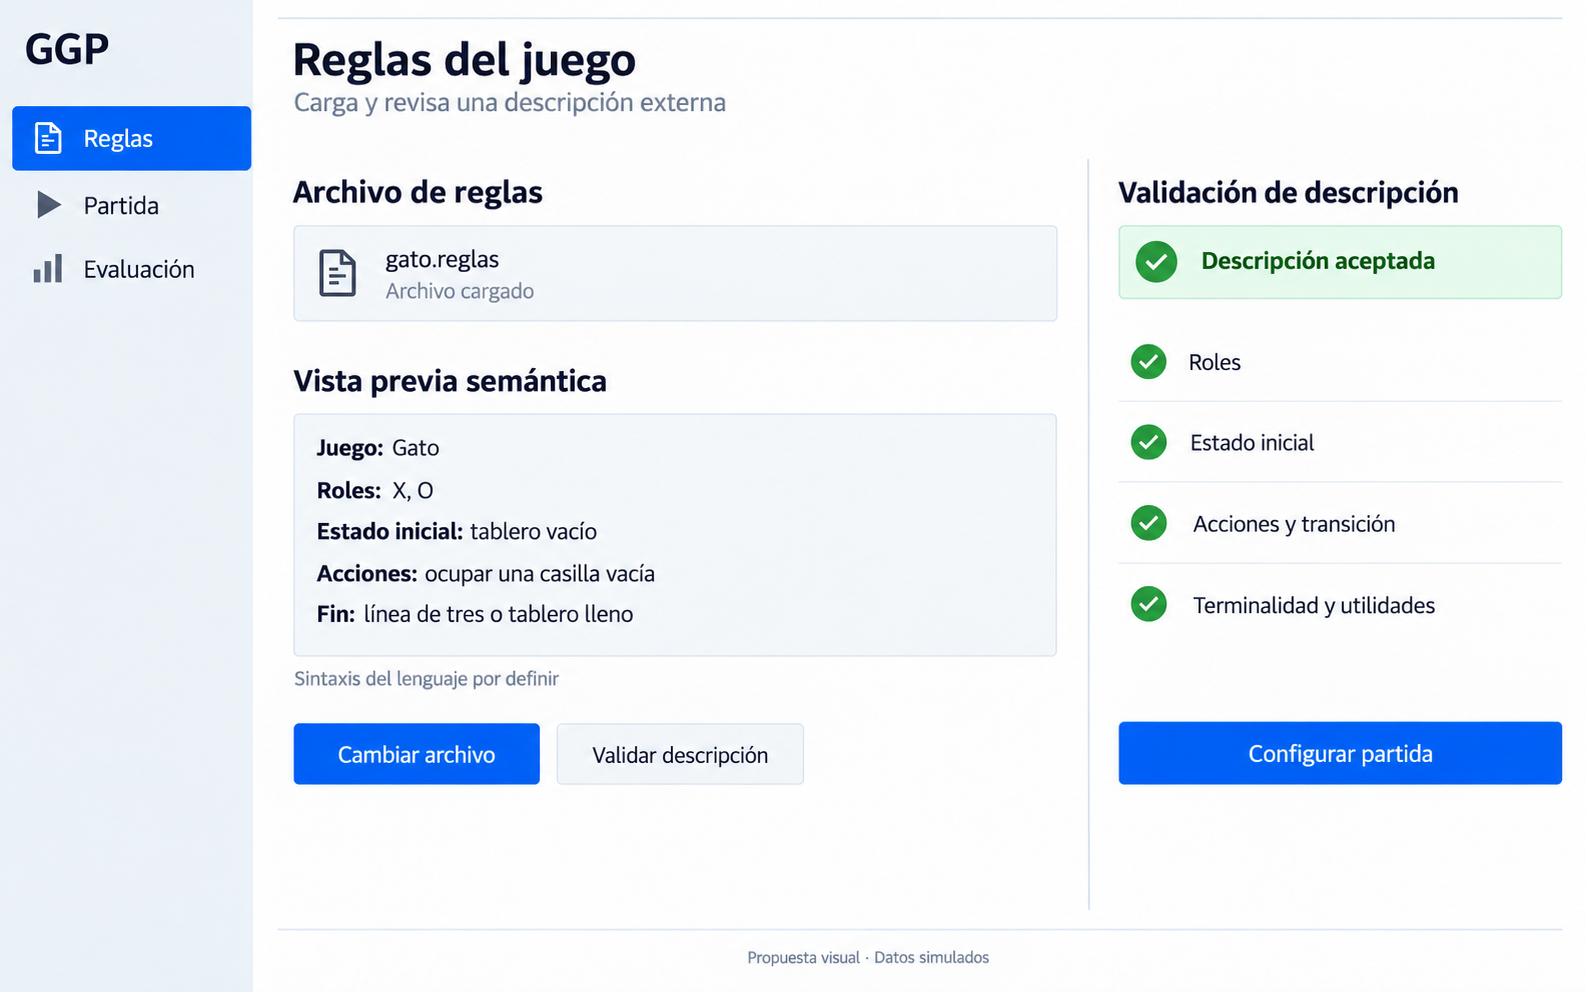
\includegraphics[width=\textwidth,height=0.80\textheight,keepaspectratio]{mockups/mockup_reglas.png}
    \caption{Prototipo aprobado de carga y revisión de una descripción externa de Gato. La validación y el contenido del archivo son ilustrativos; la sintaxis del lenguaje permanece por definir.}
    \label{fig:mockup-reglas}
\end{figure}

\paragraph{Partida de Gato.}
La Figura~\ref{fig:mockup-gato} propone una vista para una partida entre dos agentes. Presenta el tablero, el turno activo, las acciones legales, un historial y el espacio reservado para la siguiente decisión. Con ello separa la visualización de la partida de las consultas que el motor deberá resolver sobre legalidad y transición. La posición pausada y sus acciones se muestran solo como ejemplo de interacción, sin acreditar que se generen a partir de reglas ejecutables.

\begin{figure}[p]
    \centering
    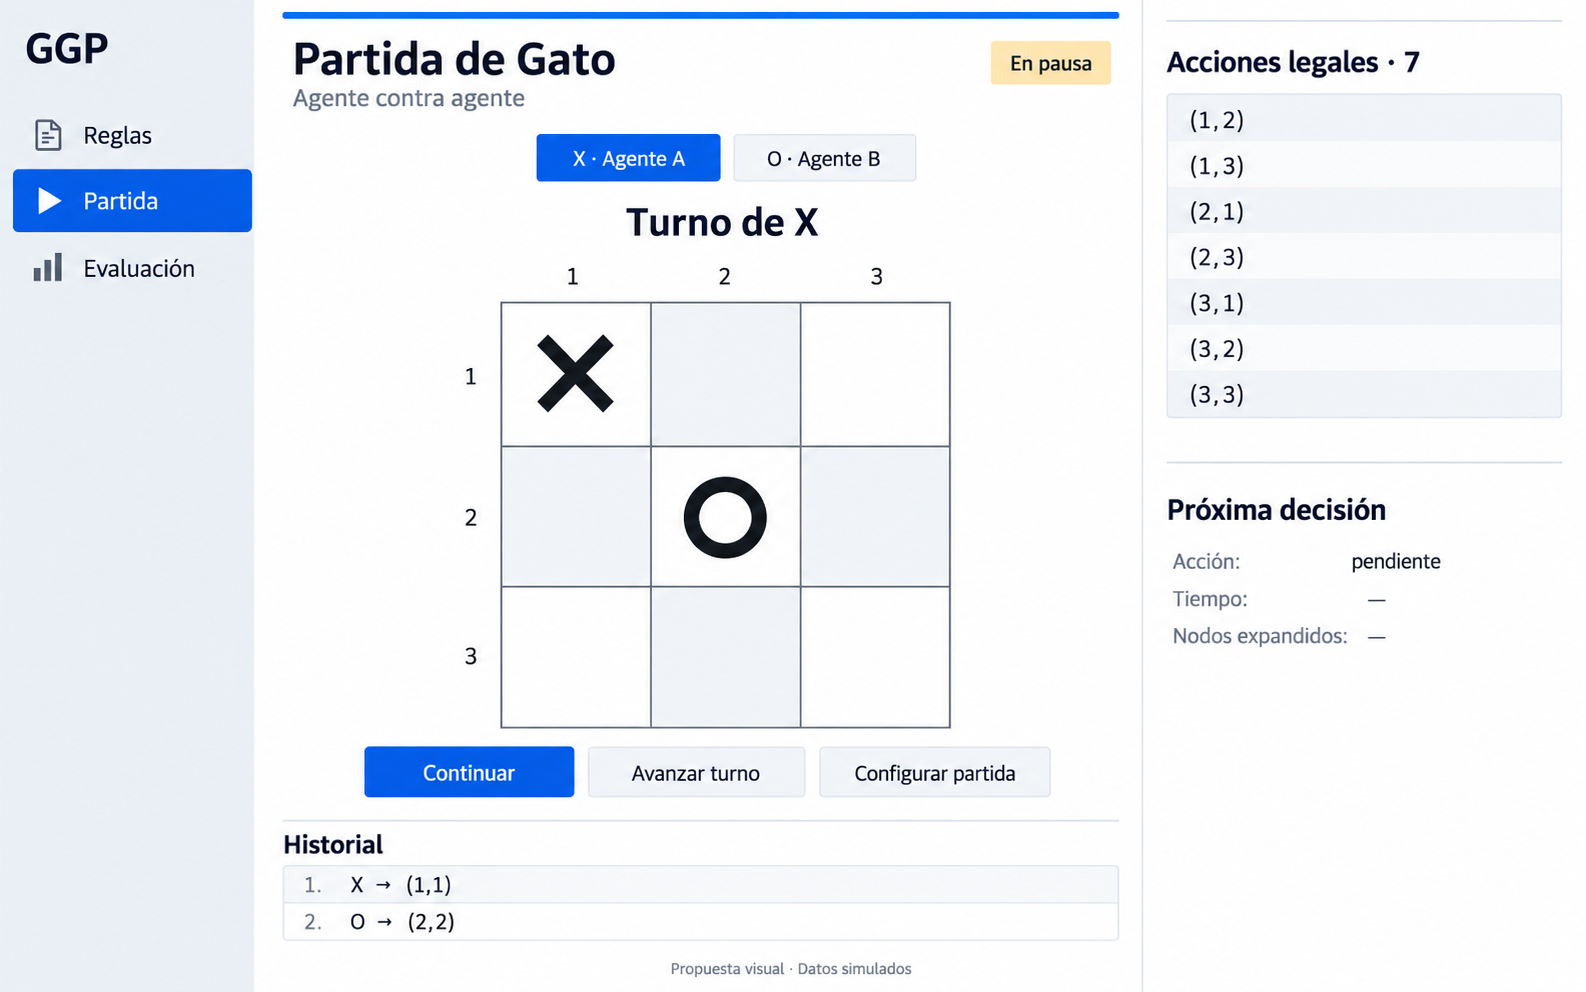
\includegraphics[width=\textwidth,height=0.80\textheight,keepaspectratio]{mockups/mockup_gato.png}
    \caption{Prototipo aprobado de una partida de Gato entre agentes. El tablero, historial, acciones legales y próxima decisión representan un estado ilustrativo.}
    \label{fig:mockup-gato}
\end{figure}

\paragraph{Partida de Ajedrez.}
La Figura~\ref{fig:mockup-ajedrez} reutiliza la misma organización para Ajedrez: tablero, turno, acciones legales, historial y próxima decisión. Su propósito es hacer visible que la interfaz no queda ligada a la geometría ni a las piezas de un único dominio; el cambio de juego corresponderá a la descripción externa y al modelo interno. La posición inicial y las veinte acciones mostradas son datos visuales de ejemplo, no una prueba de que el agente ya soporte las reglas completas de Ajedrez.

\begin{figure}[p]
    \centering
    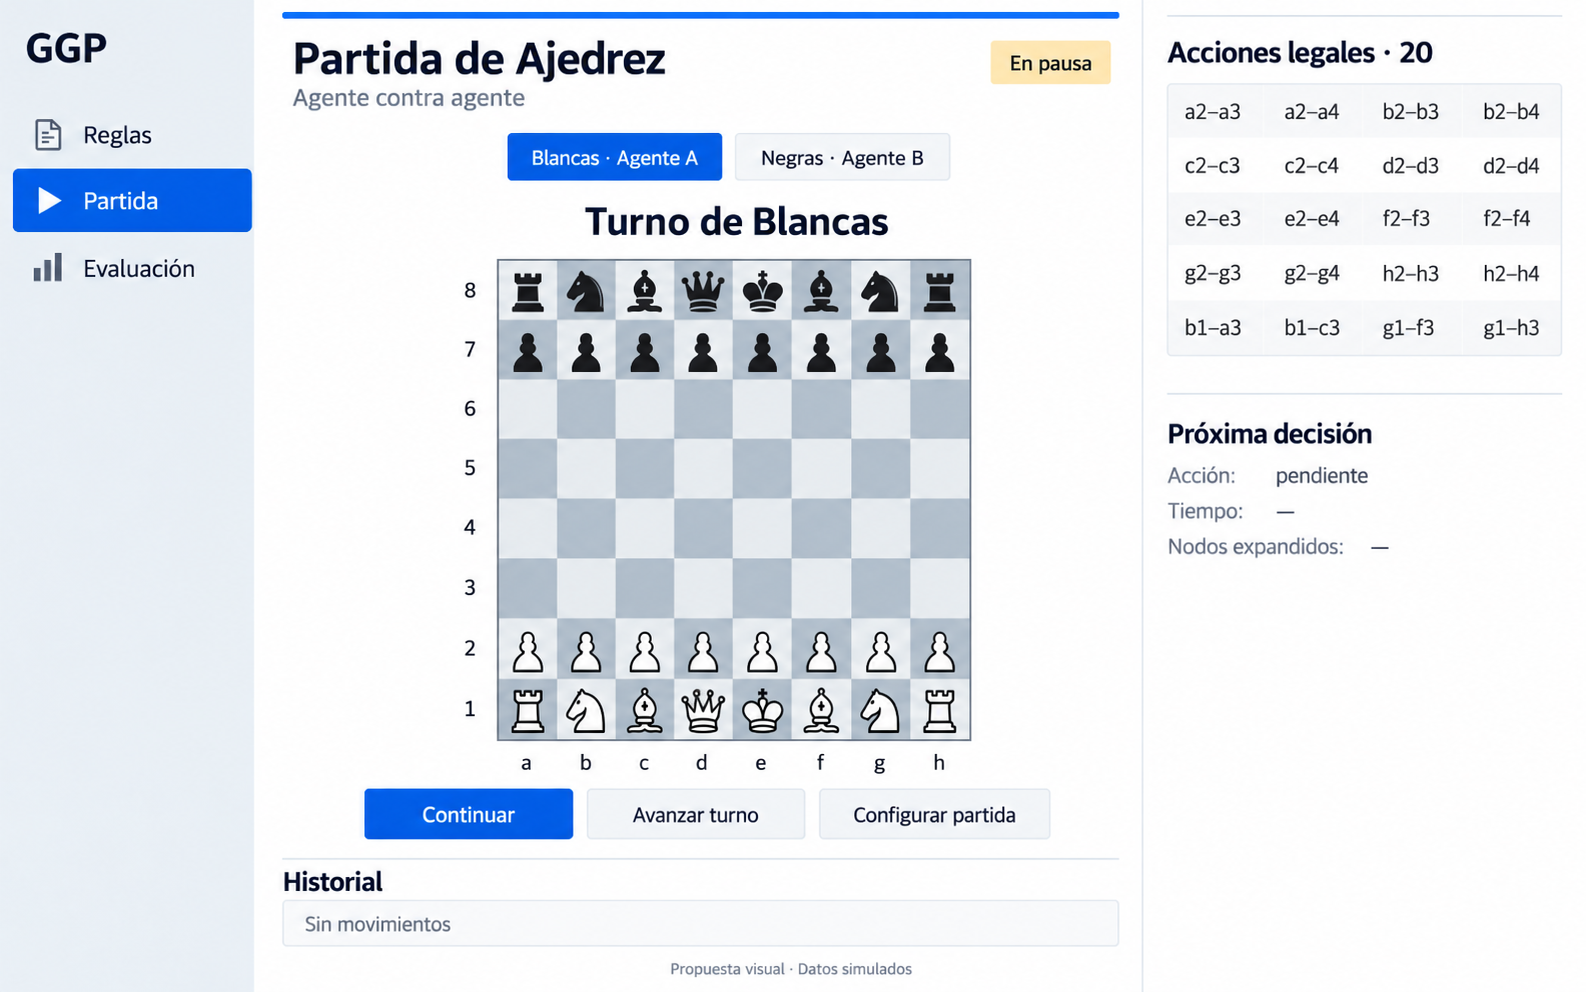
\includegraphics[width=\textwidth,height=0.80\textheight,keepaspectratio]{mockups/mockup_chess.png}
    \caption{Prototipo aprobado de una partida de Ajedrez entre agentes. La posición y las acciones son ilustrativas.}
    \label{fig:mockup-ajedrez}
\end{figure}

\paragraph{Preparación de la evaluación.}
La Figura~\ref{fig:mockup-evaluacion} representa la configuración previa de una comprobación de primera jugada en Ajedrez. Distingue el banco de casos, las condiciones de ejecución y el criterio de comparación, de acuerdo con la propuesta de métricas de la Sección~\ref{subsec:evaluacion_propuesta}. Las 30 posiciones, una ejecución por posición y el presupuesto de 1000 ms son valores de ejemplo; el tamaño definitivo del banco, las repeticiones, el presupuesto y el protocolo de Ajedrez continúan sujetos a acuerdo. La indicación de que las respuestas pertenecen al evaluador preserva la separación entre referencia independiente y agente evaluado.

\begin{figure}[p]
    \centering
    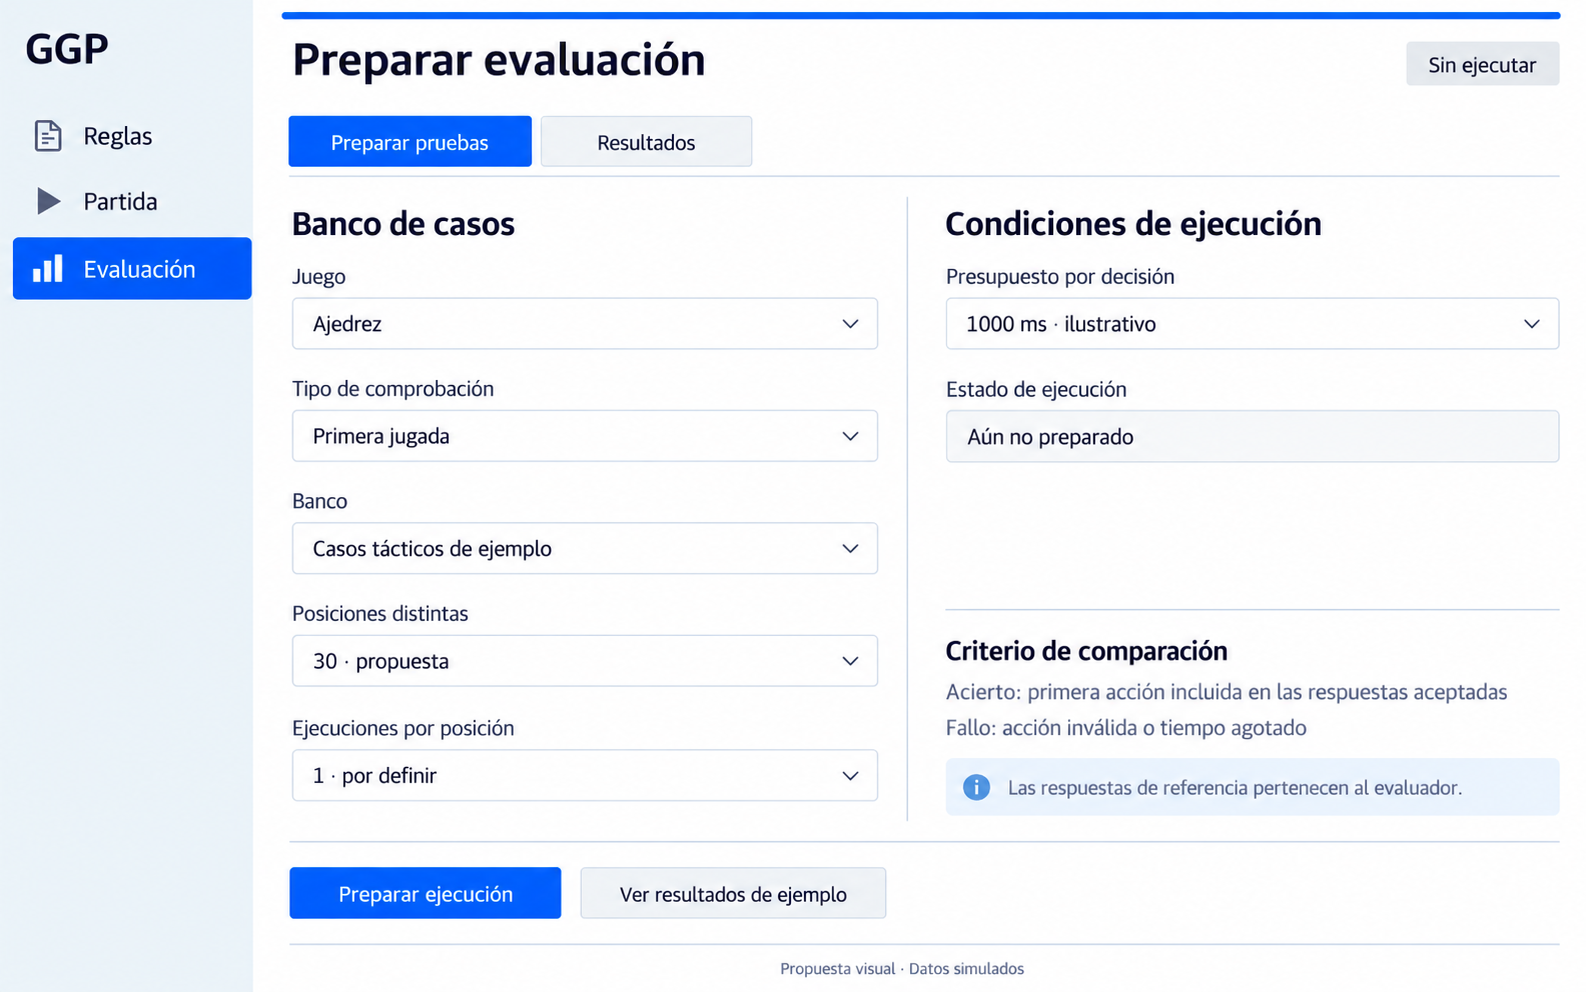
\includegraphics[width=\textwidth,height=0.80\textheight,keepaspectratio]{mockups/mockup_evaluacion.png}
    \caption{Prototipo aprobado de preparación de una evaluación táctica de primera jugada en Ajedrez. Las cantidades, el presupuesto y el estado de ejecución son ilustrativos y no describen un experimento realizado.}
    \label{fig:mockup-evaluacion}
\end{figure}

\paragraph{Resultados de evaluación.}
La Figura~\ref{fig:mockup-resultados} propone cómo reportar los indicadores definidos para la validación: acierto, tiempo por decisión, nodos expandidos, posiciones distintas, ejecuciones y detalle por caso. También conserva el motivo de terminación para que los tiempos agotados y otras incidencias permanezcan visibles en el registro. Los valores numéricos, los movimientos y el resumen de 4 de 5 casos son datos simulados; la figura no informa resultados experimentales ni selecciona un algoritmo de búsqueda.

\begin{figure}[p]
    \centering
    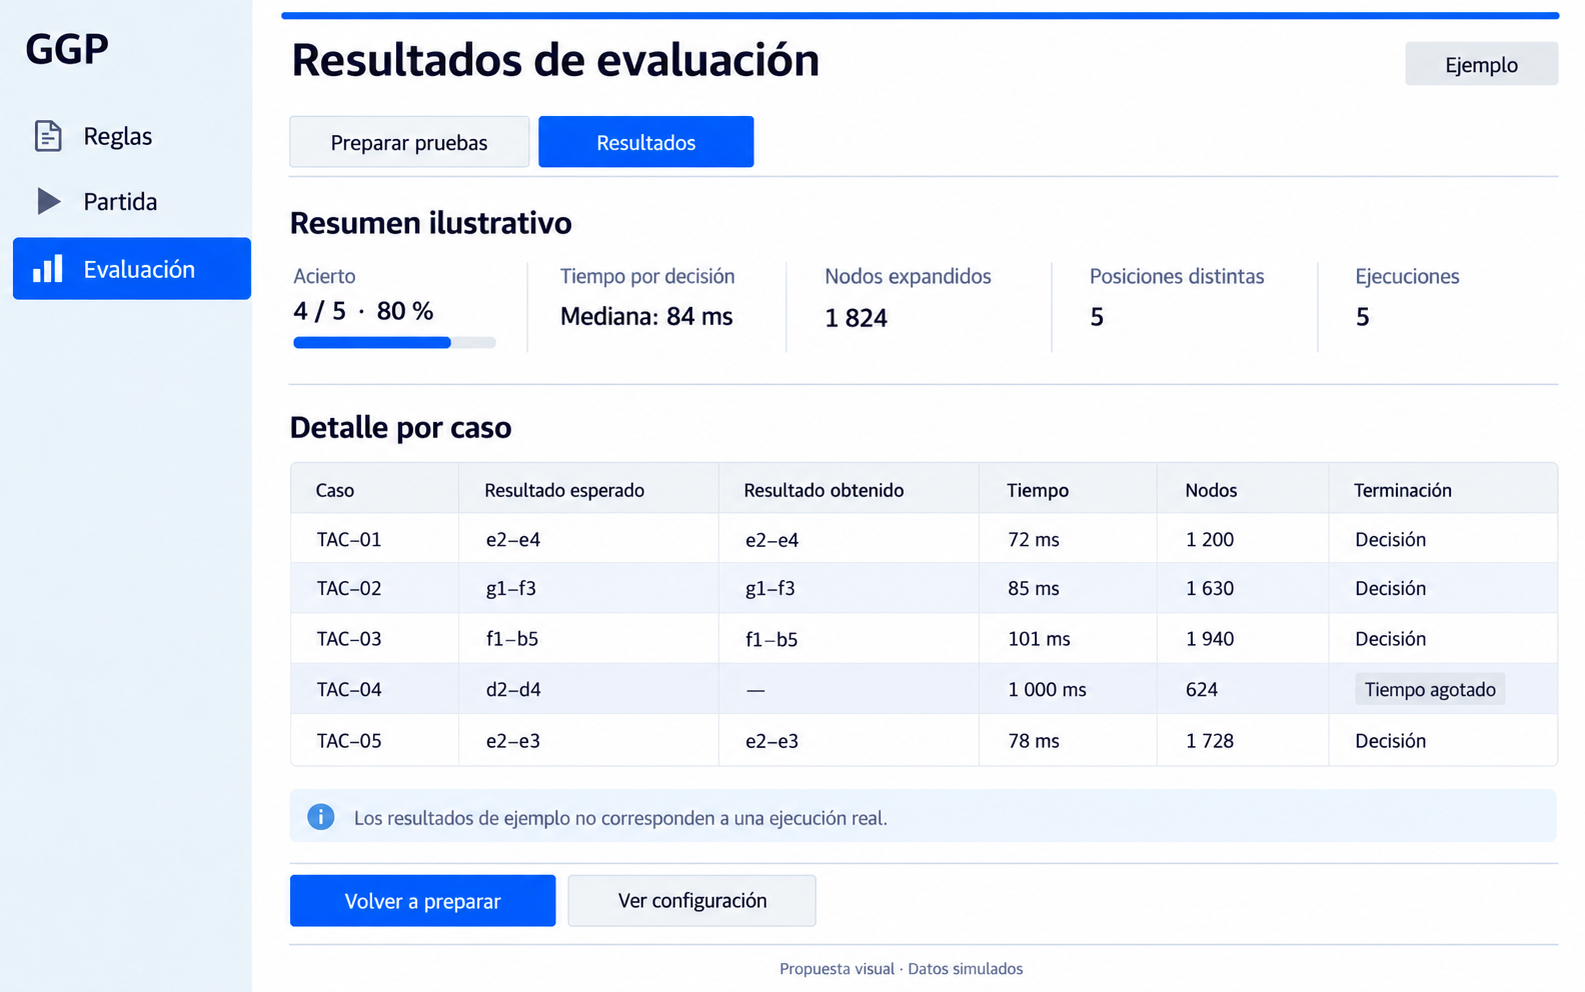
\includegraphics[width=\textwidth,height=0.80\textheight,keepaspectratio]{mockups/mockup_resultados.png}
    \caption{Prototipo aprobado del reporte de resultados de una evaluación. Las métricas y el detalle por caso muestran datos simulados, sin atribuir una ejecución real ni desempeño al agente.}
    \label{fig:mockup-resultados}
\end{figure}
